\chapter{Method}
\label{cha:method}

% In this chapter, the method is described in a way which shows how the
% work was actually carried out. The description must be precise and
% well thought through. Consider the scientific term
% replicability. Replicability means that someone reading a scientific
% report should be able to follow the method description and then carry
% out the same study and check whether the results obtained are
% similar. Achieving replicability is not always relevant, but precision
% and clarity is.
% 
% Sometimes the work is separated into different parts, e.g.  pre-study,
% implementation and evaluation. In such cases it is recommended that
% the method chapter is structured accordingly with suitable named
% sub-headings.

In this chapter, the method used is described.
Section \ref{sec:problem} formalizes the problem solved.
Section \ref{sec:environment} details the environment used to train and test an agent.
Section \ref{sec:algorithm} describes the algorithm used to train the agent.

\section{Problem Statement}
\label{sec:problem}

% and problem formulation

% environment: discrete grid
% observation: subset of grid, equals attention
% action: transform subset of grid, trigger is binary decision telling whether target is found, or whether it should be checked for thoroughly?
% reward: used to achieve correct trigger in few actions

The problem of finding an optimal sequence of actions to find can be cast as a partially observable Markov decision process (POMDP). 

Formally, we let the environment's scene be described by an \(n\)-dimensional discrete Euclidean space.
In the environment, there are \(N\) targets, each described by a subspace.
The agent observes a subspace of the state and can, though a discrete set of actions, transform this subspace.
This corresponds to changing the field of perception.
With a final action, the agent can indicate that it thinks that a target space intersects with the observed subspace.
The goal of the agent is to minimize the number of actions until all \(N\) targets have been found.

We make the assumption that the agent has knowledge of the shape of its environment's space and its current position at each time step. Using this information it can determine where it has been previously. 

% "Learning to optimize" has some good formulation tips
% explains that policy search is intractable
% Also uses a decaying step size, could be interesting for us as well
% (although we have multiple targets...)

\section{Environment}
\label{sec:environment}

In this project, we focus on search in the visual domain.
We let the state space be a three-dimensional of shape \((H, W, C)\) where \(H\) is the height of the space, \(W\) is the width of the space, and \(C\) is the number of channels in the space.
The observation space is three-dimensional of shape \((H_v, H_w, C)\).
We let the action space consist of four view-transforming actions that translate the observed subspace up, down, left or right along.
This roughly corresponds to panning and tilting a camera to look around in an environment.
It is a discretization and simplification of such a task in a 3D environment

The environments to be searched are drawn from a distribution, with varying but similar appearance, target locations and appearances.
For all environments, the appearance correlates to the probability of targets.

To incentivize finding targets quickly, the reward signal is set to -1 for each time step.
Since viewing a window twice is redundant, such actions are punished by setting the reward to -2.
If the agent selects the trigger action when a target overlaps with the window, the reward is set to 5.
When all targets have been triggered, or when 1000 time steps have passed, the episode ends.

To test the capability of the method, we use three environments of varying difficulty.
The first environment visually simple ...
The second environment is ...
The third environment consists of real images for object localization. The images are from the dataset [cite] and consists of N training samples and M test samples. Each image is 2440x2440 pixels and is therefore expensive to run object detection algorithms on. There are N training samples and M test samples.

Note that all environments are static, in that the scene is unaffected by the actions of the agent. The methods presented do, however, apply to other unknown dynamics.

% we discretize the problem
% should still apply to arbitrarily many dimensions
% assuming the existence of a suitable feature extractor

\begin{figure}
    \centering
    %% Creator: Matplotlib, PGF backend
%%
%% To include the figure in your LaTeX document, write
%%   \input{<filename>.pgf}
%%
%% Make sure the required packages are loaded in your preamble
%%   \usepackage{pgf}
%%
%% Also ensure that all the required font packages are loaded; for instance,
%% the lmodern package is sometimes necessary when using math font.
%%   \usepackage{lmodern}
%%
%% Figures using additional raster images can only be included by \input if
%% they are in the same directory as the main LaTeX file. For loading figures
%% from other directories you can use the `import` package
%%   \usepackage{import}
%%
%% and then include the figures with
%%   \import{<path to file>}{<filename>.pgf}
%%
%% Matplotlib used the following preamble
%%   \usepackage{fontspec}
%%   \setmainfont{DejaVuSerif.ttf}[Path=\detokenize{/home/oslund/.local/lib/python3.8/site-packages/matplotlib/mpl-data/fonts/ttf/}]
%%   \setsansfont{DejaVuSans.ttf}[Path=\detokenize{/home/oslund/.local/lib/python3.8/site-packages/matplotlib/mpl-data/fonts/ttf/}]
%%   \setmonofont{DejaVuSansMono.ttf}[Path=\detokenize{/home/oslund/.local/lib/python3.8/site-packages/matplotlib/mpl-data/fonts/ttf/}]
%%
\begingroup%
\makeatletter%
\begin{pgfpicture}%
\pgfpathrectangle{\pgfpointorigin}{\pgfqpoint{5.645496in}{4.234122in}}%
\pgfusepath{use as bounding box, clip}%
\begin{pgfscope}%
\pgfsetbuttcap%
\pgfsetmiterjoin%
\definecolor{currentfill}{rgb}{1.000000,1.000000,1.000000}%
\pgfsetfillcolor{currentfill}%
\pgfsetlinewidth{0.000000pt}%
\definecolor{currentstroke}{rgb}{1.000000,1.000000,1.000000}%
\pgfsetstrokecolor{currentstroke}%
\pgfsetdash{}{0pt}%
\pgfpathmoveto{\pgfqpoint{0.000000in}{0.000000in}}%
\pgfpathlineto{\pgfqpoint{5.645496in}{0.000000in}}%
\pgfpathlineto{\pgfqpoint{5.645496in}{4.234122in}}%
\pgfpathlineto{\pgfqpoint{0.000000in}{4.234122in}}%
\pgfpathlineto{\pgfqpoint{0.000000in}{0.000000in}}%
\pgfpathclose%
\pgfusepath{fill}%
\end{pgfscope}%
\begin{pgfscope}%
\pgfpathrectangle{\pgfqpoint{0.705687in}{1.624975in}}{\pgfqpoint{2.092515in}{2.092515in}}%
\pgfusepath{clip}%
\pgfsys@transformshift{0.705687in}{1.624975in}%
\pgftext[left,bottom]{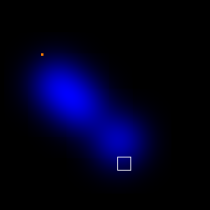
\includegraphics[interpolate=true,width=2.100000in,height=2.100000in]{environments-img0.png}}%
\end{pgfscope}%
\begin{pgfscope}%
\definecolor{textcolor}{rgb}{0.000000,0.000000,0.000000}%
\pgfsetstrokecolor{textcolor}%
\pgfsetfillcolor{textcolor}%
\pgftext[x=1.751945in,y=3.800824in,,base]{\color{textcolor}\rmfamily\fontsize{12.000000}{14.400000}\selectfont SearchGaussian-v0}%
\end{pgfscope}%
\begin{pgfscope}%
\pgfpathrectangle{\pgfqpoint{2.988431in}{1.624975in}}{\pgfqpoint{2.092515in}{2.092515in}}%
\pgfusepath{clip}%
\pgfsys@transformshift{2.988431in}{1.624975in}%
\pgftext[left,bottom]{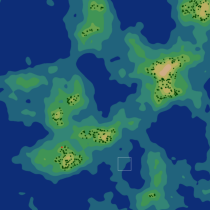
\includegraphics[interpolate=true,width=2.100000in,height=2.100000in]{environments-img1.png}}%
\end{pgfscope}%
\begin{pgfscope}%
\definecolor{textcolor}{rgb}{0.000000,0.000000,0.000000}%
\pgfsetstrokecolor{textcolor}%
\pgfsetfillcolor{textcolor}%
\pgftext[x=4.034689in,y=3.800824in,,base]{\color{textcolor}\rmfamily\fontsize{12.000000}{14.400000}\selectfont SearchTerrain-v0}%
\end{pgfscope}%
\begin{pgfscope}%
\pgfpathrectangle{\pgfqpoint{0.705687in}{0.469634in}}{\pgfqpoint{0.951143in}{0.951143in}}%
\pgfusepath{clip}%
\pgfsys@transformshift{0.705687in}{0.469634in}%
\pgftext[left,bottom]{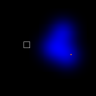
\includegraphics[interpolate=true,width=0.960000in,height=0.960000in]{environments-img2.png}}%
\end{pgfscope}%
\begin{pgfscope}%
\pgfpathrectangle{\pgfqpoint{1.847059in}{0.469634in}}{\pgfqpoint{0.951143in}{0.951143in}}%
\pgfusepath{clip}%
\pgfsys@transformshift{1.847059in}{0.469634in}%
\pgftext[left,bottom]{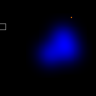
\includegraphics[interpolate=true,width=0.960000in,height=0.960000in]{environments-img3.png}}%
\end{pgfscope}%
\begin{pgfscope}%
\pgfpathrectangle{\pgfqpoint{2.988431in}{0.469634in}}{\pgfqpoint{0.951143in}{0.951143in}}%
\pgfusepath{clip}%
\pgfsys@transformshift{2.988431in}{0.469634in}%
\pgftext[left,bottom]{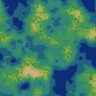
\includegraphics[interpolate=true,width=0.960000in,height=0.960000in]{environments-img4.png}}%
\end{pgfscope}%
\begin{pgfscope}%
\pgfpathrectangle{\pgfqpoint{4.129803in}{0.469634in}}{\pgfqpoint{0.951143in}{0.951143in}}%
\pgfusepath{clip}%
\pgfsys@transformshift{4.129803in}{0.469634in}%
\pgftext[left,bottom]{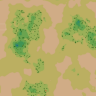
\includegraphics[interpolate=true,width=0.960000in,height=0.960000in]{environments-img5.png}}%
\end{pgfscope}%
\end{pgfpicture}%
\makeatother%
\endgroup%

    \label{fig:environments}
    \vspace*{-1cm}
    \caption{Samples from each environment.}
\end{figure}

\section{Algorithm}
\label{sec:algorithm}

% self-supervised pretraining?
% https://arxiv.org/pdf/2003.14323.pdf

The agent is trained with reinforcement learning using Proximal Policy Optimization with function approximation using neural networks. 

% section 17.4 in sutton is good!

% https://xbpeng.github.io/projects/DeepMimic/index.html

% reward shaping: change reward signal as agent progresses
% could also shape the environment itself, make it more and more difficult
% each modification should be made so that the agent frequently receives reward with its current policy
% this is what we do when we train animals! ie give treats to dogs
% why isn't this working...

% reward normalization: 
% reward clipping: done in "playing atari with deep reinforcement learning": they state that since the scale of scores varies from game to game they fix all positive rewards to be one and negative to be -1. 0 rewards are left unchanged. this limits the scale of the error derivatives and makes it easier to use the same learning rate across multiple games. could also affect agent's performance as it cannot distinguish between rewards of different magnitudes.
% could be important for us if the number of targets and the reward varies a lot

\section{Architecture}

% resnets?
% https://efficientdl.com/how-to-train-a-resnet-efficiently/

% should use a constant network architecture

The architecture of the neural network is presented in Figure X.

The network is split into three main section: the feature extraction, the shared network, and the policy and value heads.
Like Mnih et al., we use a CNN~\cite{} for feature extraction.
The shared network consists of an LSTM~\cite{hochreiter}.
Finally, both the policy and the value head are two-layer MLPs.

% Actor critic

% Feature extraction
% Shared Network
% Policy Head
% Value Head

% we should clearly explain the thought process
% connect back to local search problems
% we need a good feature extraction
% and then something for a belief state
% finally, what is the idea behind policy and value (should be in theory instead)

\section{Implementation}

The environment is implemented with Gym~\cite{gym}, and the agent is implemented with PyTorch~\cite{pytorch}. 

% we could give some pseudocode here

\section{Experiments}

The first environment was used to determine a good observation space.
By just observing the current window, the agent can never learn a suitable policy to solve the problem.
This is because it cannot distinguish between equal windows at different locations.
Experiments are run with several additional observation types: window position, ...
Results of these experiments are presented for this environment only.

The agent was trained using the algorithm described in Section \ref{sec:algorithm} for 100 million time steps in all three environments using PPO, PPG and A2C.
Hyperparameters are tuned with random search separately for each environment.
For all experiments, the average return per episode is reported together with the theoretically optimal reward (obtained with an optimal path).
The agent was trained and tested on the full distribution of environments.

With the best performing algorithm we compare three different reward signals.
One gives a constant time penalty of -1 to incentivize finding the target quickly.
The second gives a constant time penalty of -2 and an exploration bonus of +1 when a new view is reached.
The third gives a reward of +1 for moving closer to the target and a penalty of -1 otherwise, as in \cite{caicedo_active_2015}.

Additionally, experiments to eveluate the generalization capability of the agent were conducted.
These were conducted on the procedurally generated terrain environment following the approach suggested in ~\cite{procgen}.
During training, the seed pool size was fixed to various sizes to limit the training set size.
The agent was trained for varying number of timesteps and then tested on the full distribution of environments.
This way, we can get a sense of how much data and simulation is required to use the approach for real-world tasks.

All experiments are conducted on an Intel Core i9-10900X CPU and an NVIDIA GeForce RTX 2080 Ti GPU.

For each experiment, we report the mean return and episode length over time during training.
We compare the approach to an exhaustive search and a human searcher with prior knowledge of the characteristics of the searched environments.
As per [rlliable], we report results across multiple seeds.

% learning actions, recognition and localization simultaneously feels in itself interesting
% how do we interpret such a model? are there papers for visualizing reinforcement learning weights

% detailed
% replicability

% pre-study
% implementation
% evaluation

% discuss state representation
% need more than the image
% - either memory or position or both

% seed + 1000 levels training
% >= s + ... for test
% do the same as procgen

% also same configuration possibly?
% more parallel environments seem to lead to stable training (relatively slow increase in reward though...)

% would be nice to have a varying number of targets
% also a done action
% measure false positives, false negatives etc.
% good replacement for zoom?
% relates to visual search literature
% the current setup is also the most natural for a computer vision system
% foveated vision is not very reasonable


% select one algorithm and clearly motivate why!
% probably PPO, but why?


% time to find targets could be measured in terms of execution time, 
% and number of timesteps. this way, it could be easier to incorporate 
% visual attention if it is deemed reasonable.

% how do we handle appearance of targets:
% can an agent learn to recognize anything out of the ordinary?
% maybe not the focus, but just the search

% an interesting question is how large search windows we can handle
% could be an alternative to zoom
% a large search window presumably requires attention


% memory is needed for (a) remembering previous locations, and (b) integrating features over time


% PPO
% PPG
